%!TEX root = report.tex

\chapter{Travail Accompli}
\section{Introduction du chapitre}
Dans ce chapitre on procéde à la presentation des cas utilisateur de notre systéme ainsi que l'identification des acteurs impliqué dans ces cas. Puis on décortique l'implementation que nous proposant en citant eventuellement nos motifs et intentions.

\section{Vue Général}
\subsubsection{Identification des acteurs}
Notre systéme interagie essentiellement avec trois acteurs différents:
\begin{description}
\item[Le medecin] C'est l'acteur principale de notre systéme.

\item[Le service web] Source des données à achiminé vers le medecin
(Tache et )

\item[Systéme d'exploitation] Communique à notre systéme les information
receuille des divers composants qui nous interresse (localisation
GPS/Network, etat de la connectivité, etat de la battery).

\end{description}

\subsection{Cas d'utilisations}

\begin{figure}
\center
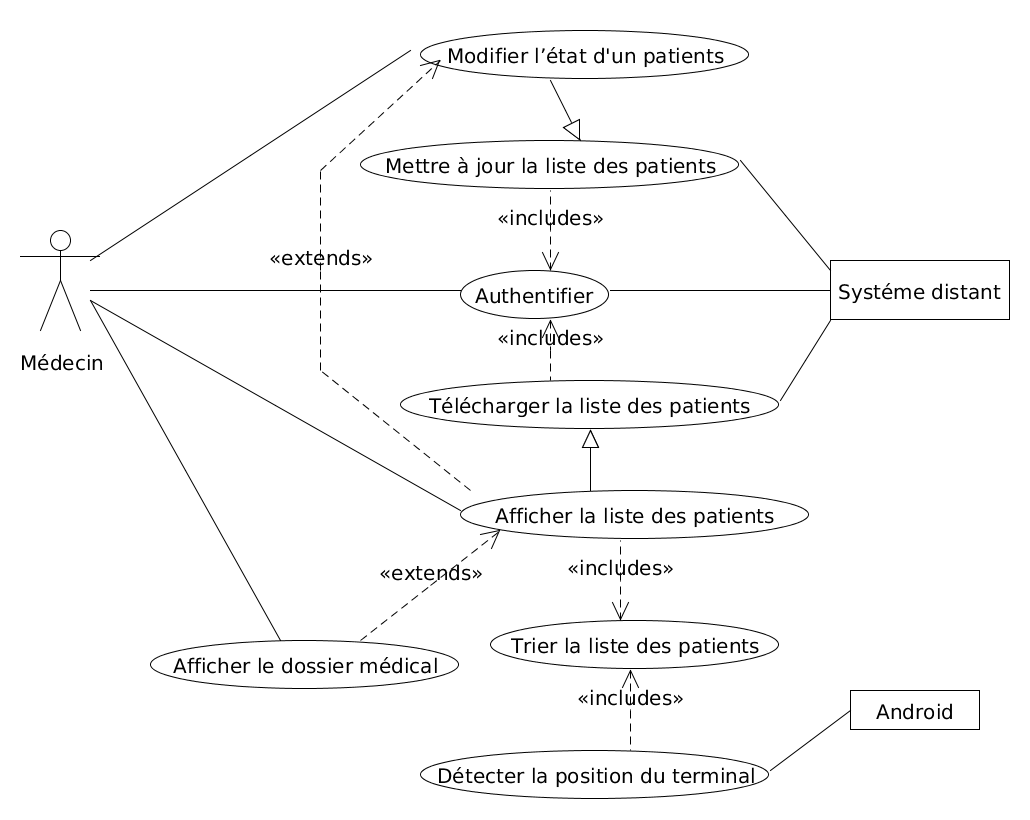
\includegraphics[width=0.8\textwidth]{diagrams/usecases}
\caption{Diagramme \gls{uml} des cas d'utilisation.}
\label{fig:usecase}
\end{figure}

\subsubsection{Cas: Authentifier}
\subsubsection{Cas: Notifier la proximiter d'un patient}
\subsubsection{Cas: Detecter la position du terminal}
\subsubsection{Cas: Afficher la list des patients}
\subsubsection{Cas: Télecharger la list des patients}
\subsubsection{Cas: Modifier la list des patients}
\subsubsection{Cas: Mettre à jour la list des patients}

\subsection{Environnement de développement}%TODO

\section{Architecture Général}

\begin{figure}
\center
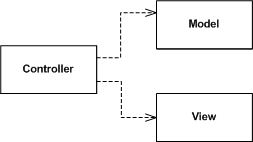
\includegraphics[scale=1]{passive_view}
\caption{Diagramme \gls{uml} du patron \en{Passive Viev}~\cite{fowler:passive_view}}
\label{fig:passive_view}
\end{figure}

L'architecture globale de l'application est calqué sur Le patron "Vue
Passive" (Passive View). Le patron \en{Passive View} (fig
\ref{fig:passive_view}) est une variation des patrons \gls{mvc} et
\gls{mvp}, à ce qui ce passe dans ces patrons l'interface utilisateur
est divisé entre une vu qui s'occupe de l'affichage des données et un
controlleur qui repont aux interactions de l'utilisateur. La différance
majeur avec le \en{Passive View} est que la vue est completemement
passive et n'ai pas responsable de sa mise à jour depuis le model. Dans
ce cas tout la logique de la vue est dans le controlleur et aucune
dependances ni dans un sens au dans un autre entre le vue et le
model~\cite{fowler:passive_view}.

Ce patron est idéal dans notre cas pour deux raisons majeurs:
\begin{itemize} 

\item Dans notre projet le en{view} n'est pas une partie très important
dans la mesure ou l'objectif est d'intégré un système éventuellement
pré-conçu, donc avec une autre logique de présentation. Déporter les
interactions avec le modèle dans le contrôleur permet d'intégrer
d'autre implémentation d'affichage plus facilement.

\item La nature même de cette procédure d'accés - a savoir l’aspect
abstrait, donc plus fragile - nous pousse à réduire les composants en
relations pour réduire la marge d'erreur possible et facilité les tests.

\end{itemize} 

Dans la suite de ce chapitre, on procède à l'explication détaillés de chaque composant de cette architecture.

\section{Le Modèle} 


Un des objectifs de ce projet étant de fournir une solution d’accès au
donnée flexible à fin de couvrir les besoins de chaque client de manière
individuel. On a opter donc pour un modèle basé sur l’implémentation de
deux interfaces (figure \ref{fig:adl}):

\begin{itemize}
\item Interface d'authentification.
\item Interface d’accès à la liste des patients.
\end{itemize}

\begin{figure}
\center
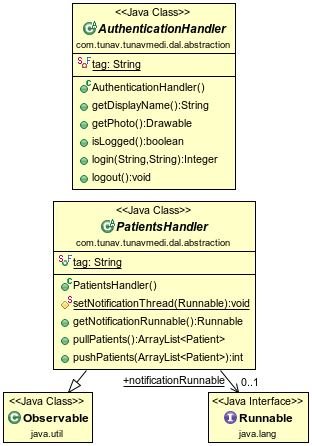
\includegraphics[width=0.8\textwidth]{diagrams/cls_adl}
\caption{Diagramme de classe de la couche d'accées.}
\label{fig:adl}
\end{figure}

L'idée est simple: pour chaque client, une implémentation spécifique à son infrastructure sera développez soit par son propre effectif, soit par une des équipes de Tunav, ou dans le cas idéale par une alliance formé par des agents des deux camps qui garantie une collaboration plus poussée pour des résultats meilleurs.
Ces ensemble d'interfaces nous permet de construire notre application 

\subsection{Implémentation de test} 

\begin{figure}
\center
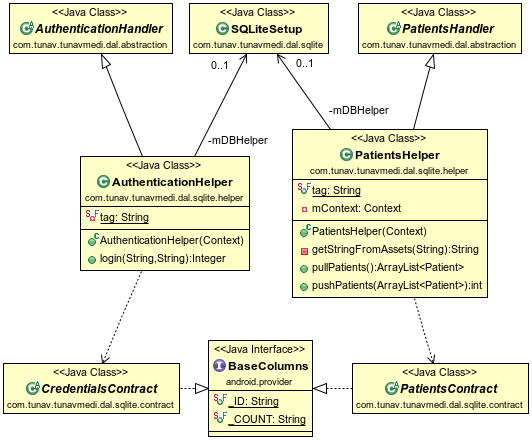
\includegraphics[width=0.8\textwidth]{diagrams/cls_adl_sqlite}
\label{fig:adl_sqlite}
\caption{Diagramme de classe de l'implémentation de la couche d'accées de test à base de SQLite.}
\end{figure}

Une implémentation de la couche d’accès abstraite est réalisé dans le
cadre de ce projet pour pouvoir testé la solution. Cette implémentation
est de caractère locale à l'application à travers les \gls{api} de la
base de données \dev{SQLite} qui fait parti de l'\gls{sdk} \android{}.
En fait une implémentation locale nous affranchies des problèmes qui
peuvent se produire dont la corrélation avec l'application est faible.
Cette même idée a influencé la mise en place même de cette
implémentation qui à su rester la plus simple possible en restant très
proches des objets de base de notre application.

Se trouvant dans le package \dev{com.tunav.tunavmedi.dal.sqlite}, cette implémentation peut être subdivisé en trois éléments:

\begin{description}
\item[Les Contrats] représente les contrats relative aux tables dans notre implémentation de test. chaque contrat implémente l'interface \dev{android.provider.BaseColumns} et contient - entre autre - les commandes SQL de création et de suppression de la dite table, des éventuel index, et les commande d'insertion des données de test.

\item[Les \en{Helpers}] ce sont les implémentations des classes
abstraites qui définisse la couche d’accès et présente les procédure d'extraction des données pré-inséré dans nos table fictives en faisant appel à la classe \dev{SQLiteSetup} .

\item[la classe \dev{SQLiteSetup}] Elle hérite de la classe \dev{SQLiteOpenHelper} et destiner à contrôler la création et l’accès à notre base de données de teste.
\end{description}

\subsection{Interface d'authentification}

\subsection{Interface des Données}
\subsubsection{Mécanisme de notification}

\begin{figure}[H]
\center
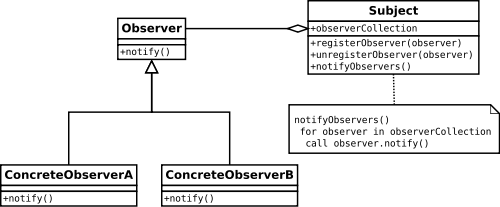
\includegraphics[width=0.8\textwidth]{Observer}
\caption{diagramme UML du patron de conception Observateur~\cite{wiki:observer}}
\label{fig:observer}
\end{figure}

Le patron \textbf{Observateur} (\en{observer pattern}) (fig \ref{fig:observer}) et un patron de conception couramment utilisé et qui nous perment d'avoir une relation 1/N entre divers objets.
Le patron observateur assume que l'objet qui contient les données est séparé des l'objets qui les affiche et ces dites objets \en{observe} le changement de ces données~\cite{jdp-observer}.
Quant on implémente le patron observateur, on réfère communément à l'objet contenant les données par "Sujet"; et chacun des consommateurs des données par "Observateur", Et chaque Observateurs implémente une interface préconnu que le Sujet invoque quant les données changes~\cite{jdp-observer}.
Dans le langage Java, ce patron est réaliser à travers la class \dev{java.util.Observable} et l'interface \dev{Java.util.Observer}. Le Sujet hérite de la classe \dev{Observable} et les changements sont signalé par les méthodes \dev{setChanged()} et \dev{notifyObservers()} ou \dev{notifyObservers(Object message)}.

%TODO show in our code

\section{Le Contrôleur}

\section{La Vue}
Le système d'exploitation \android rend facile le développement des application qui tourne sur des appareils qui possèdes des forme et des taille d’écran différents, une des amélioration

\section{Testes}

\subsection[Pourquoi tester?]{Pourquoi tester? ~\cite{pycon:getting_started_with_automated_testing}}

\begin{itemize}
\item La raison la plus évidente pour écrire les testes - étant la plus populaires aussi - est que c'est un moyen efficace pour savoir si le bout de code ajouté dans le projet marche correctement ou pas, ce qui non seulement fournit une certaine confiance dans la robustesse du logiciel mais présente un effet secondaire bénéfique en réduisant le temps nécessaire pour le débogage à la recherche d'un bug caché. %FIXME
\item Une autre raison pour écrire les testes est que c'est un autre forme de documentation qui aide les autres développeurs comprendre le code contenu dans le projet.
\item Une raison non évidente pour écrire des teste est le fait que les tests améliore la manière dont le code est conçu en mettant en évidence les difficultés pour le maintenir.
\end{itemize}
\subsubsection{Modifié la localisation dans l'émulateur}%FIXME

\subsection{Quelque difficultées rencontrées}

\section{Conclusion du chapitre}